\section{Generation of Calibrated Radiances}
\label{sec:5.2:CalibratedRadiances}

ALI arrived back in Saskatoon on September 25, of 2015 and was unpacked and checked for any damages from either the transportation back to Saskatoon or from the landing at the end of the mission. No obvious damage had occurred to ALI and the instrument was functioning correctly. This allowed the complete data set record by ALI to be downloaded and used for aerosol profile processing. This section will undergo the method used to convert the raw data from the CCD to measured relative radiances used in the retrieval process.

The raw flight data, known as the level 0 data, must be converted to into level 1 relative radiances, which is the data normalized to a laboratory measurement value, before they can be used to retrieve aerosol extinction and particle size. The transformation includes removal of dark current, DC bias, stray light, and application of flat fielding calibration.

The DC offset is an bias that is applied to the analogue digital converter inside the CCD camera that causes a bias in the final count values for the image. This need to be removed in order to be able to get the pure measurement counts from the instrument. It is usually assumed that the DC offset for a CCD is a constant across the operating temperatures and exposure times of the device, however the DC offset for the camera used in ALI exhibited a temperature dependance. By using the dark images from the assent of the flight which was in darkness combined with laboratory dark images all of which were takeing at the shortest possible exposure time of the camera, 0.01~s, to remove contribution from dark current. For all the images in the data set the mean value of the counts was used for each image across the whole image. For each each the standard deviation of the counts ended up being 2 to 3 percent of the average value. Using this data a curve was fit to determine the DC offset with respect to temperature and the curve is in the form of
\begin{equation}
    \text{DC offset} = 0.00659T^{3}-0.09202T^{2}-3.5368T+643.5127
    \label{eqn:5.2:DcOffsetCurve}
\end{equation}
where $T$ is the CCD temperature as measure from the CCD temperature sensor in degrees Celsius and is plotted in \autoref{fig:5.2:dcOffsetCurve}. The dark current is the thermal energy that builds up in the CCD pixels that grows linearly with exposure time and temperature. For the operating temperatures of ALI combined with the short exposure times used during the mission lead to the system having a very small dark current contribution in the measurement images. The dark current was as small as a single count to at most seven counts for the worst case scenario (longest exposure time and hottest temperature.) Since this correction was small compared to the DC offset and the final measurement counts the dark current was added as a a noise contribution for the images. At this point all the non-exposure time sensitive components had been removed and all the images were converted from counts to counts per second by divided the corrected counts by the exposure time.
 %by taking the counts in the image and divided by the exposure time, in order to easily relate the radiance of different images directly to each other without having to scale the results with respect to the exposure time.

\begin{figure}
    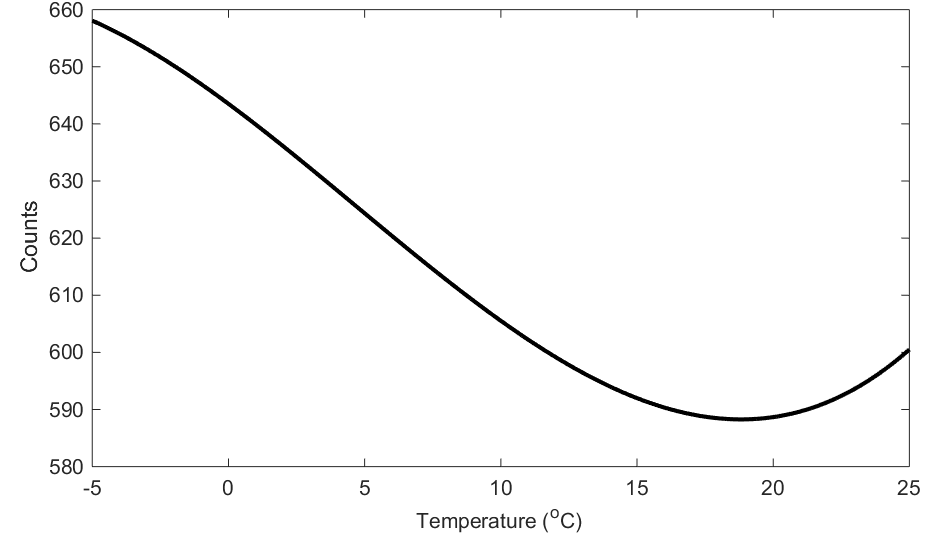
\includegraphics[width=1.0\textwidth]{./Images/5-2-DcOffset.pdf}
    \caption[Determined ALI DC Offset]{The determined DC offset determined for ALI in the form seen in \autoref{eqn:5.2:DcOffsetCurve}. The counts on the vertical axis os the counted that need to be removed to remove the DC offset.}
    \label{fig:5.2:dcOffsetCurve}
\end{figure}

Stray light removal has always been difficult in atmospheric instrumentation due to the difficulty in accurately discerning the signal in regards to the stray light contamination. Furthermore, ALI's optical system has the further addition of unwanted light internal to the instrument because of the rejection of one of the polarizations due to the nature of the AOTF. The signal enters the optical system unpolarized, but only one polarization can have a consistent output angle from the AOTF. The entering light is passed through a linear polarizer with an extinction ratio of at least 100,000:1 to remove the unwanted polarization however a small percentage is not absorbed. Furthermore, a second linear polarizer is used after the AOTF to reject all of the unwanted radiance that did not meet the Bragg criteria and once again a small percentage of this radiance is not absorbed. Since only a very small wavelength bandpass composses the wanted signal even small component of the unwanted signal passing through the system adds a considerable amount of stray light. However, the active filtering of the AOTF allows for an image to be measured when the filtering device is disabled, which is with no applied RF, allowing only the stray light to be captured by the instrument which will be referred to as a `dark image'. During ALI's aerosol mode a `dark image' was captured before every measurement image. By removing the `dark images' from the signal-stray light contaminated images the end result is images that only contain the measured signal. The previous method was tested in the lab, a 250~W quartz-tungsten light source was passed through a dispersing screen and into the entrance aperture of ALI filling the entire field of view. Using variety of exposure times ranging from 0.1~s to 60~s and wavelengths from 650 to 950~nm in 25~nm internals the incoming source was imaged twice for each unique combination; one image recorded with the AOTF in its off state, with no driving RF wave, and one with the ATOF in its on state, with the RF wave. Once all the images were acquired the DC offset was removed and the counts were divided by the exposure times to give counts per second. Essentially, the image with the AOTF off only contains stray light in the system, as previously stated, and the AOTF on image contains the stray light combined with the even signal from the light source. By subtracting the AOTF off image from the AOTF on image results in an image that just contains the signal and the contamination from the stray light from the system have been removed. Using the images from the experiment the bright areas over the smooth background of the AOTF on images could be successfully removed by subtracting the AOTF off image leaving a resulting image that contains a bright centre with the a smooth fallout in brightness, which is due to the known vignetting of the system. In order to be able to uses this method during the campaign all images captured in the standard aerosol mode will have a corresponding AOTF off or `dark image' recorded as well. An example from the mission with the stray light removal method being preformed is located in \autoref{fig:5.2:strayLightComparison} where the features cause by the stray light are sen to be removed in the final image.

\begin{figure}
    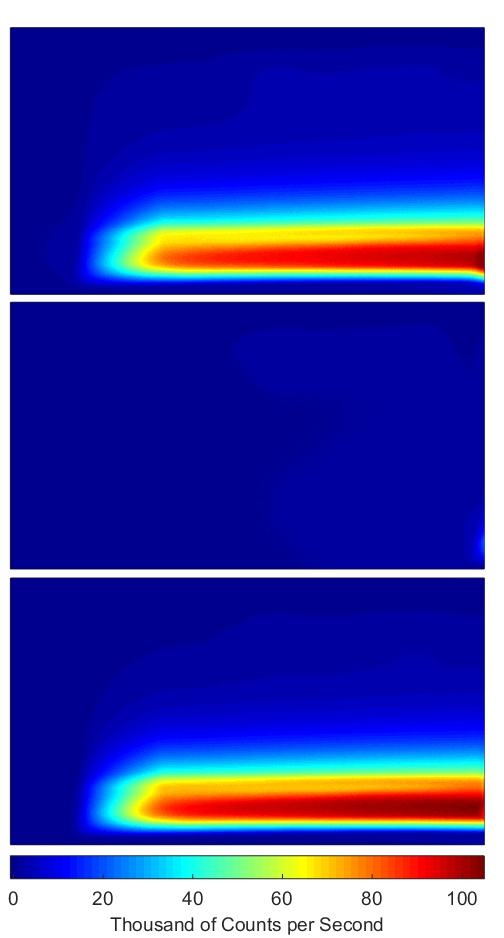
\includegraphics[width=0.5\textwidth]{./Images/5-2-StrayLightComparison.pdf}
    \caption[Example Stray Light Removal]{An demonstration of the stray light removal method will be preformed using image 208 from the Timmins campaign, which is a 750~nm measurement. The top panel is the image after the DC offset has been removed from a measurement image and in the top right the gradient in the blue raises much higher than in the left portion of the measurement. The middle panel is the associated `dark image' with the AOTF off and the same feature can be seen in the upper right of the image as well as light being registered in the entire right hand portion of the image which should be dark, this is the stray light that is coming into contact with the CCD. The final panel is the the middle panel minus the top panel and the abnormal gradient has been removed from the final image, leaving a clean radiance profile.}
    \label{fig:5.2:strayLightComparison}
\end{figure}

The vignetting is caused by the aperture of the AOTF itself, by using a simple optical layout as chosen for the prototype the larger the angle for the field of view the more light that get blocked by the AOTF's aperture causing a known vignetting for the images. Furthermore the extreme range of the field of view, approximately the last one degree in each direction, is outside the acceptance angle of the AOTF which causes a loss of diffraction efficiency. Both of these effect will also need to be calibrated out of the measurements to achieve final level 1 radiances. To finalize the data into level 1 relative radiances a flat fielding calibration is preformed which is done in two steps: first the images are flat fielded spatially for each wavelength, and second the images are flat fielded over the wavelength range to remove different efficient for different wavelength in the ALI system. In order to determine the coefficients, the final images from the stray light lab test will be used. To determine the spacial flat fielding coefficients the images were sorted into each specific wavelength. Flat fielding coefficients was determined for each pixel in a wavelength set but before starting the analysis, since the images were recorded at various exposures times some images had low signal and some had high signal as such any pixels that were below the noise threshold for the DC offset and completely filled the CCD well were removed for the analysis. Using the rest of the images a coefficient was determined for each pixel of each image to normalize the value of counts per second for every pixel in the form
\begin{equation}
    f_{\lambda, i, j, k} = \frac{c_{ave, k}}{c_{\lambda, i,j , k}}
\end{equation}
where $f_{\lambda, i, j, k}$ is the flat fielding coefficient for a specific pixel location , $i,j$, for for a specific trial image in the wavelength, $k$, $c_{ave, k}$ is the average of the center 25 by 25 pixels of the trial image, and $c_{\lambda, i,j , k}$ is the counts per second of the pixel. Over all images in the average pixel value was always with 3\% of the median value for all images. For each wavelength the value of the average flat fielding coefficients, $f_{\lambda, i, j}$ that was used as the final value and a 3\% error was added to the final counts per second to each pixel. An example of the flat fielding coefficients for the 750~nm wavelength can be seen in \autoref{fig:5.2:flatFieldCoeff}. To achieve the flat field images for each wavelength the following was preformed on the mission data
\begin{equation}
    \mathbf{I}_{\lambda} = \mathbf{C}*\mathbf{F}_{\lambda}
\end{equation}
where $\mathbf{C}$ is the stray light corrected image form the mission, $\mathbf{F}_{\lambda}$ is the matrix of flat fielding coefficients, and $\mathbf{I}_{\lambda}$ is the flat fielded values.

\begin{figure}
    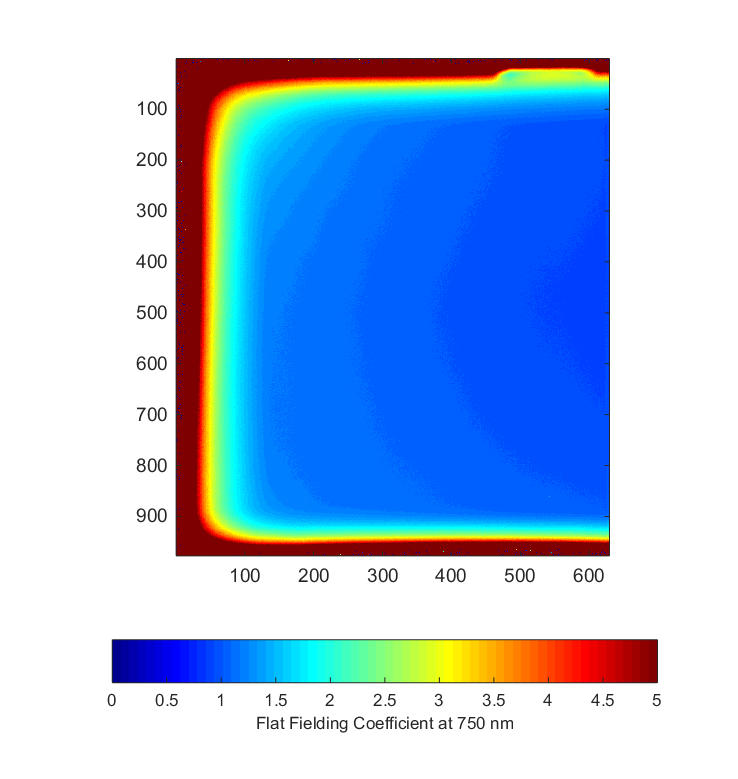
\includegraphics[width=1.0\textwidth]{./Images/5-2-FlatFieldCoeff.pdf}
    \caption[750~nm Flat Feilding Coefficients]{The flat fielding coefficients, $\mathbf{F}_{\lambda}$ for 750~nm. Due to the vignetting the the values near the edge require the largest flat fielding value but a majority of the image has a scaling factor of approximately unity. }
    \label{fig:5.2:flatFieldCoeff}
\end{figure}

Once the normalization numbers across the spacial direction had been preformed, a similar methods was done for the spectrally as well. For this method, the average of the 25 by 25 pixel area used for the spacial flat fielding were used again to determine the spectral calibration curve from the specially calibrated data. This curve is simple and the coefficients are given by
\begin{equation}
    g(\lambda) = \frac{I_{ave}(\lambda_{ref})}{I_{ave}(\lambda)} 
\end{equation} 
where $g(\lambda)$ is the scaling factor for the spectral range of ALI, $I_{ave}(\lambda_{ref})$ is the average over the center 25 by 25 pixels of the reference the wavelength, and $I_{ave}(\lambda)$ average the of 25 by 25 pixels at a specific wavelength $\lambda$. The percent errors of the determined $g(\lambda)$ and $I_{ave}(\lambda_{ref})$ are 2\% and 1\% respectively across the entire wavelength band. The reference wavelength is 775~nm since it is the wavelength that ALI is most sensitive. The calibration coefficient $g{\lambda}$ and the final flat fielding calibration for a mission image is
\begin{equation}
    \mathbf{I(\lambda)} = \frac{\mathbf{C}*\mathbf{F}_{\lambda}*g(\lambda)}{I_{ave}(\lambda_{ref})}.
\end{equation}
The final radiance $\mathbf{I(\lambda)}$ is called a relative radiance since it normalized to the 775~nm lab radiance value.

A completed calibration from a raw level 0 image to a level 1 relative radiance measurement can be seen in \autoref{fig:5.2:BeforeAfterImages} and the loss of brightness form the edge portion of the images have been removed and the image has a smooth profile horizontally across the entire field of view. However the noise level for individual pixel were large and in order to increase the precision of the measurements from the flight the images were averaged in cells of 25 horizontal pixels and vertical pixel averaging that would result in the measured radiances being on a 1~km vertical grid. Furthermore, a loss of resolution was speculated to occur in the flight data because of the drastic change in temperature of the optics during the flight which is a secondary reason for the pixel averaging. ALI radiance profiles from the complete mission from the 0\si{\degree} line of sight can be seen in \autoref{fig:5.2:AliRadiancesVectors} which includes wavelengths from 675-950~nm and generally have good internal agreement from 13 to 30~km. A spectrum of relative radiances are shown at a series of altitudes using the measurements from images 204 to 216 in \autoref{fig:5.2:AliSpectralRadiances}. Images 207, 211, and 215 were selected to demonstrate subtle radiance differences between different horizontal lines of sights with each profile's respective error and can be seen in \autoref{fig:5.2:AliRadiances}. 

\begin{figure}
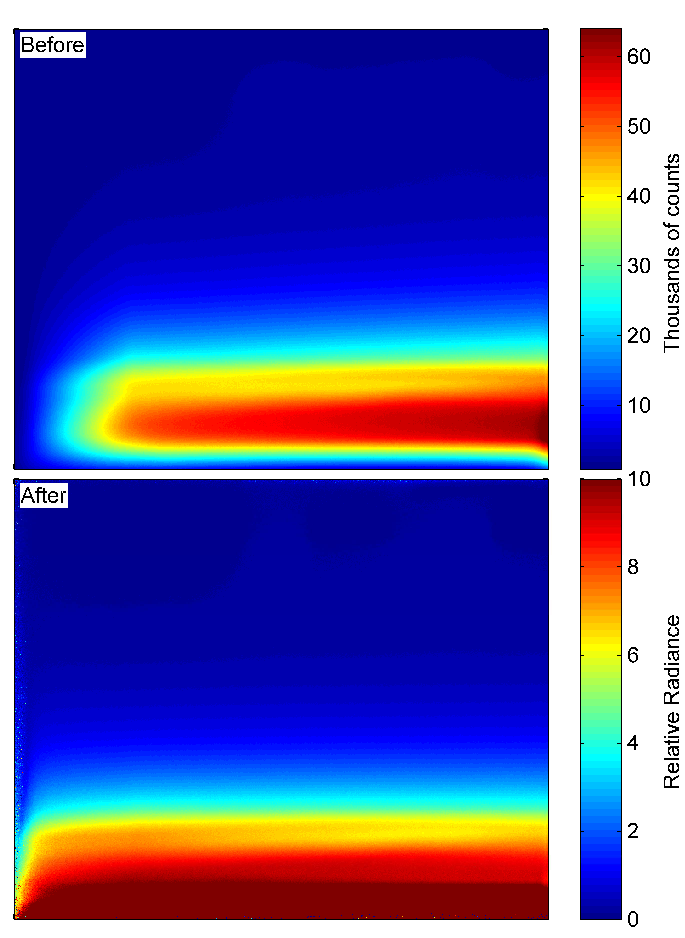
\includegraphics[width=1.0\textwidth]{./Images/5-2-BeforeAfterImage.pdf}
    \caption[Comparison of an Raw and Calibrated ALI Image]{Comparison of the same image, image number 212, at 750~nm. The upper panel is the raw level 0 data and the lower panel is the relative radiance level 1 data.}
    \label{fig:5.2:BeforeAfterImages}
\end{figure}

\begin{figure}
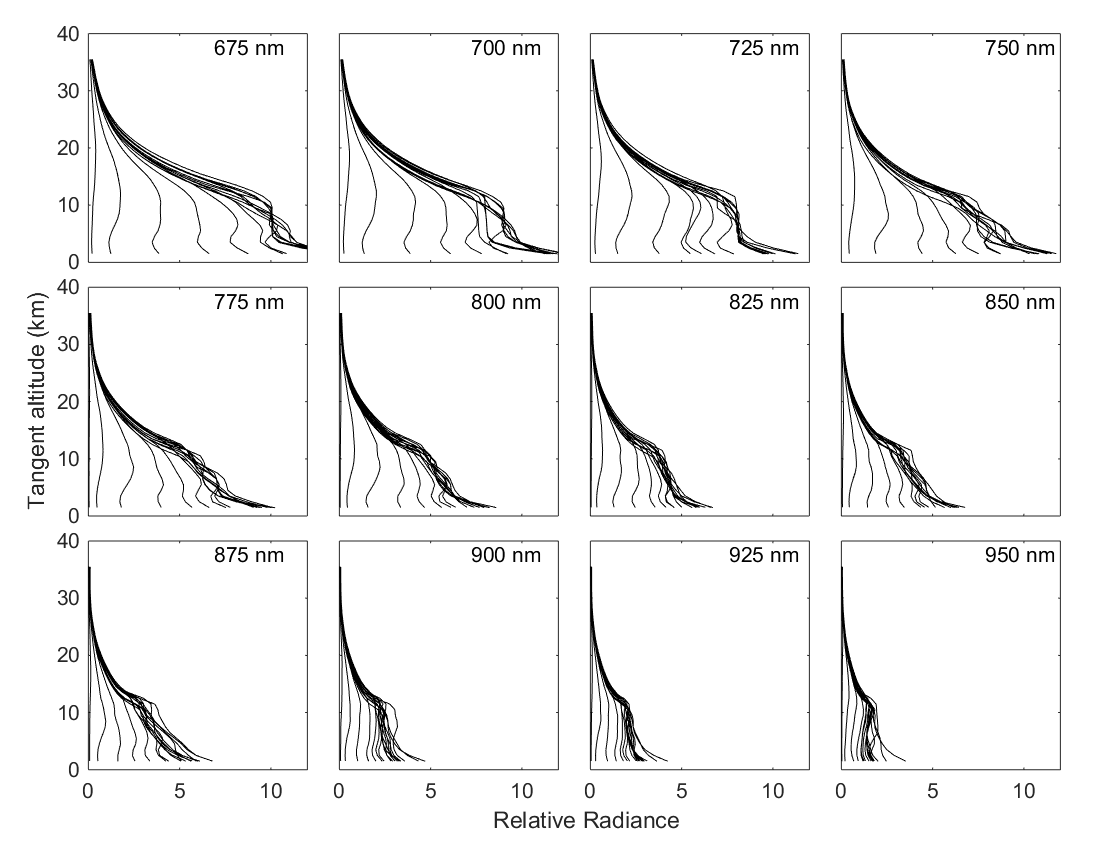
\includegraphics[width=1.0\textwidth]{./Images/5-2-AliRadianceVectors.pdf}
    \caption[ALI Relative Radiance Vectors]{All ALI relative radiance vectors from the NIMBUS-7 flight from the straight ahead line of sight, the average of the centre 25 columns of pixels, averaged to a 1~km resolution. Each panel presents the radiance vectors from a different wavelength measured which is denoted in the top right corner.}
    \label{fig:5.2:AliRadiancesVectors}
\end{figure}

\begin{figure}
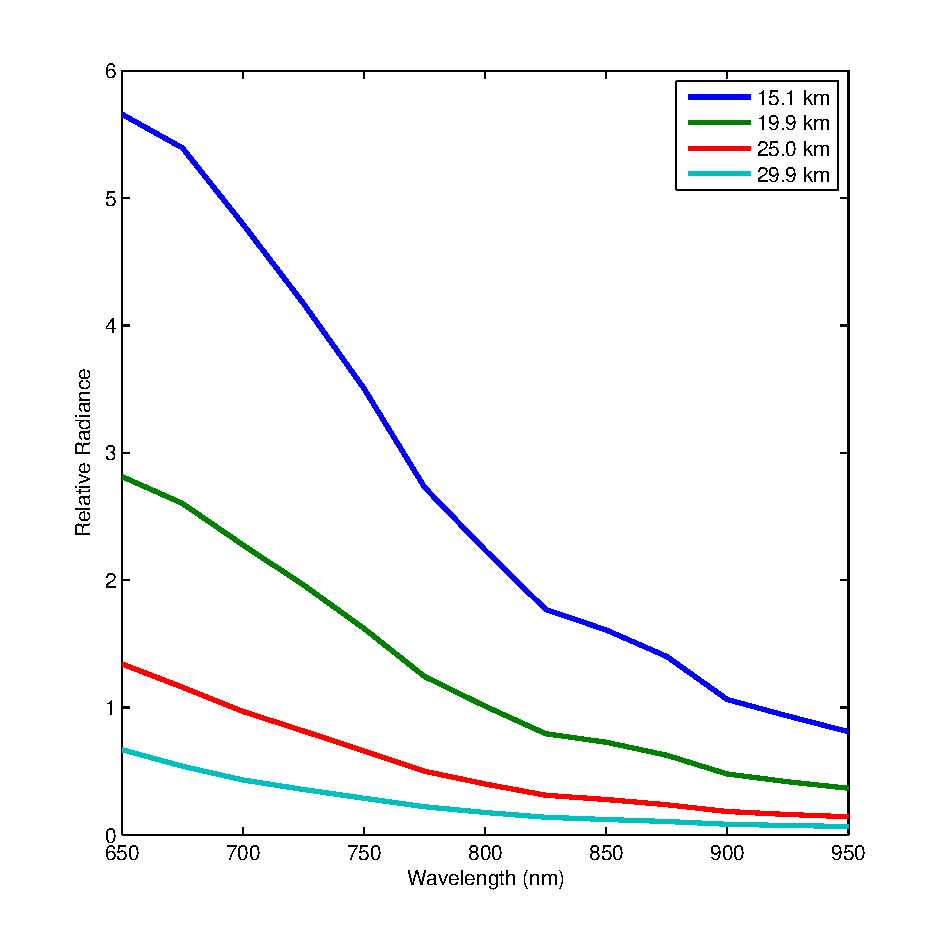
\includegraphics[width=1.0\textwidth]{./Images/5-2-AliSpectralRadiances.pdf}
    \caption[ALI Spectral Relative Radiance]{Level 1 relative radiances spectrally from 650~nm to 950~nm as measured form ALI at approximately 14:20 UTC consisting of images number 204 to 216 looking 90\si{\degree} from the sun facing southwards. These spectral profiles are presented at several tangent altitudes with a horizontal field of view of 0\si{\degree}.}
    \label{fig:5.2:AliSpectralRadiances}
\end{figure} 

The final step in determining the relative radiances is to determine the error on the profiles. Each step in the calibration has an associated error that gets added to the final result. The first step is to analysis the error contributed form the camera readout and DC offset and dark current removal, if the raw image from the CCD is $\mathbf{R}$ with elements $R_{i,j}$ and $\mathbf{C}_{raw}$ is the image with the DC offset, and dark current removed then the error contribution would be given by
\begin{equation}
    \delta\mathbf{C}_{raw}^2 = \frac{\delta\mathbf{R}}{t} = \frac{\delta\mathbf{e}_{r}^{2} + \delta\mathbf{e}_{DC}^{2} + \delta\mathbf{e}_{dark}^{2}}{t}
\end{equation}
where $\delta \mathbf{e}_{r}$ is the read error from the camera which is listed to be 15 counts, $\delta \mathbf{e}_{DC}$ is the error cause by the DC offset which was determined from the calibration via the standard deviation to be approximately 30 counts, $\delta \mathbf{e}_{dark}$ us the error added from the dark current removal which is 5 counts at worse, and $t$ is the exposure time. The same method is used for the `dark image' and the final result is denoted $\mathbf{C}_{stray}$. At this point each image has its stray light removed with a `dark image' subtraction yielding an error of
\begin{equation}
  \delta\mathbf{C} = \delta\mathbf{C}_{raw} + \delta\mathbf{C}_{stray}.
\end{equation} 
The final error is added via the flat fielding process yielding the final error on each image
\begin{equation}
    \delta\mathbf{I(\lambda)} = \frac{\delta\mathbf{C}\mathbf{F}_{\lambda}g(\lambda)}{I_{ave}(\lambda_{ref})} + \frac{\mathbf{C}\delta\mathbf{F}_{\lambda}g(\lambda)}{I_{ave}(\lambda_{ref})} + \frac{\mathbf{C}\mathbf{F}_{\lambda}\delta g(\lambda)}{I_{ave}(\lambda_{ref})} + \frac{\mathbf{C}\mathbf{F}_{\lambda}g(\lambda)\delta I_{ave}(\lambda_{ref})}{I_{ave}(\lambda_{ref})^{2}}.
\end{equation}
This error was rather large for analysis and was reduced by the averaging of pixels together. As mention earlier the image was banned into 25 horizontal bins and a vertical resolution to yield results on a 1~km grid. In order to determine the final error from the relative radiance the error must be combined from the following
\begin{equation}
    \delta I_{final}(\lambda) = \frac{(\Sigma^{n}_{i}\Sigma^{m}_{j}\delta I(\lambda)_{i,j}^{2})^0.5}{nm}
\end{equation}
where $i$ and $j$ is the index of horizontal and vertical pixel locations and and $n$ and $m$ are the number of pixels to be summed horizontally and vertically respectively. The final binned relative radiance profiles with the associated error for three horizontal field of vie can be seen in \autoref{fig:5.2:AliRadiances}.

%and used to normalized the full field of view across the whole spectrum to the center of the 750~nm images, thus giving a relative calibration of radiance referenced to this point. The process used to determine the flat fielding coefficients started with similar process used to remove the stray light during the mission post processing. The images had the DC bias and dark current removed for proper unbiased comparisons and converted to counts per second. Each value of every pixel in the active region of the CCD was normalized to the mean of the value on the center 25 by 25 pixels at 750~nm over all exposure times and trials. The coefficients for flat fielding can be determined as the values to yield a unified radiances of one across all field of views and wavelengths. These coefficients are then applied to the data from the flight that give relative radiances for each pixel.

\begin{figure}
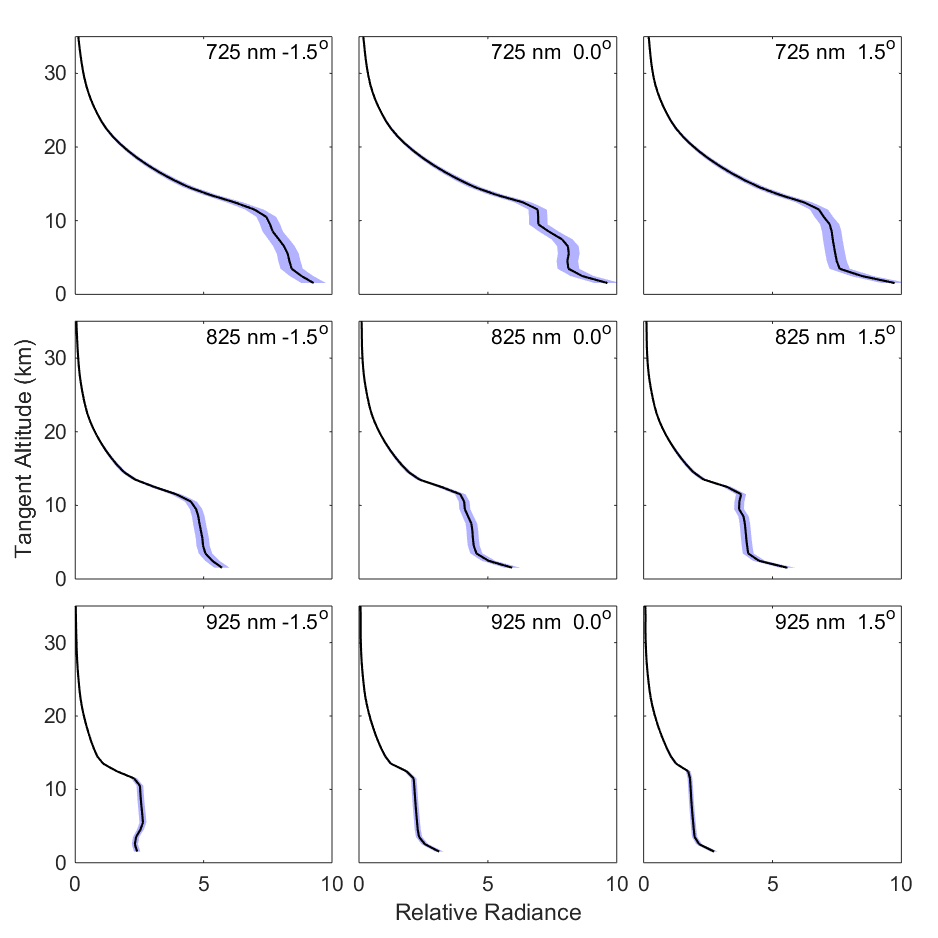
\includegraphics[width=1.0\textwidth]{./Images/5-2-AliRadiancesWithError.pdf}
    \caption[ALI Relative Radiance Vectors with Error and Horizontal Variance]{Level 1 relative radiances as measured from ALI at approximately 14:20 UTC (images number 207, 211,and 215) looking 90\si{\degree} from the sun facing southwards. The top, middle, and bottom rows are measurements taken at 725, 825, and 925~nm respectively and each row is comprise from a single image with a different horizontal line of sight with the respective calibration and readout error shown by the blue shading. The center column is viewing the atmosphere with a 0\si{\degree} line of sight, while the left column is looking to the left at -1.5\si{\degree} and the right at 1.5\si{\degree}. The difference in the radiance profiles demonstrates ALI sensitivity to horizontal distributions in atmospheric composition, specifically aerosol.}
    \label{fig:5.2:AliRadiances}
\end{figure}
